\graphicspath{{figure/chap2/}}
\chapter{光的干涉}
\section{杨氏双缝干涉}
用两个点波源作光的干涉实验的典型代表是杨氏双缝实验.

\insertfig{2-1.png}{杨氏双缝实验示意图}{0.7}

在普通单色光源前面放一个开有小孔$S$的屏, 作为单色点光源. 在$S$的照明范围内再开放一个开有小孔$S_1$和$S_2$的屏. 按照惠更斯原理, $S_1$和$S_2$作为两个次波源向前发射次波(球面波), 形成交叠的波场. 在较远的地方放置一接收屏, 屏上可以观测到一组几乎是平行的直线条纹. 设从$S$到$S_1$,$S_2$的距离为$R_1$,$R_2$, 光源$S$发光时的随机相位为$\varphi_0(t)$,$S_1$和$S_2$两个次波源的相位差为:
\[
\Delta \varphi_0 = \frac{2\pi}{\lambda}(R_2-R_1) +\varphi_0(t)-\varphi_0(t) = \frac{2\pi}{\lambda}(R_2-R_1)
\]

注意到随机相位在相减中被消去, 保证了两束光分开后相位差的稳定性. 像这样, 将一束光通过装置分为两条传播路径, 从而实现空间中的交叠和干涉, 这种干涉被称为分波前(波阵面)的干涉.

\insertfig{2-2.png}{杨氏双缝实验结果}{0.5}

如图所示, 光程差可以被表示为:
\[
\delta = r_2 - r_1 \approx d \sin \theta, \quad x =L\tan\theta \approx L \sin \theta \Rightarrow \delta = d \frac{x}{L}
\]

对于光强, $I_1 = I_2 = I_0 $,$\Delta \varphi(P) = \frac{2\pi}{\lambda} d\sin\theta$这样我们得到之前的光强表示公式为:
\[
I = I_1 + I_2 + 2\sqrt{I_1 I_2} \cos(\Delta \varphi(P)) = 2I_0+2I_0 \cos\left(\frac{2\pi}{\lambda} d \sin \theta \right) = 4I_0\cos^2\left(\frac{\pi}{\lambda} d \sin \theta \right)
\]

根据用光程差表示的干涉条件, 我们可以得到:
\[
\begin{cases}
d \frac{x}{L} = k \lambda, & k \in \mathbb{Z}, \quad \text{干涉极大} \\
d \frac{x}{L} = (k - \frac{1}{2}) \lambda, & k \in \mathbb{Z}, \quad \text{干涉极小}
\end{cases}
\]

于是得到明纹和暗纹中心的位置为
\[
\begin{cases}
x = \pm k\frac{L}{d}\lambda ,& k \in \mathbb{N}, \text{明纹中心}\\
x = \pm(k - \frac{1}{2})\frac{L}{d}\lambda, & k \in \mathbb{N}^{*},\text{暗纹中心}
\end{cases}
\]

相邻的明(暗)条纹间距为:
\[
\Delta x = \frac{L}{d}\lambda
\]

以上我们讨论的是单色光的干涉. 如果光源中包含着两种波长的谱线, 那么屏幕上将会存在两套间距不等的干涉条纹.

在讨论干涉装置的时候, 我们往往会关心如下一些特征:
\begin{itemize}
    \item 相位差的计算公式;
    \item 条纹的特点: 包括级次分布, 中心条纹位置, 条纹间距等等;
    \item 条纹的决定因素, 变化特点等.
\end{itemize}

因此, 现在我们来探讨杨氏双缝实验中干涉条纹的移动. 造成条纹移动的因素一般有三种, 一是光源的移动, 二是装置结构的变化, 三是光路中介质的变化.

探讨干涉条纹的变动时通常可以用两种方式提出问题, 一种是固定场点$P$, 考察有多少条干涉条纹移过该点, 另一种是跟踪干涉场中某一级条纹, 例如0级条纹, 看其朝什么方向移动了多少距离. 对于前一种情况, 我们需要考察交于该点的两条相干光线之间的光程差的表达式, 每当光程差变化一个波长时, $P$点就会有一条干涉条纹移过. 对于后一种情况, 我们需要计算出该条纹的光程差, 然后考察具有该光程差的场点的去向.

\begin{noteenv}
    我们来看看轴上点源移动对干涉条纹的影响. 初始状态下零级条纹位于$O$点, 光程差为零. 现在将点源$Q$向$x$轴正方向移动了$x_0$, 其造成的干涉条纹, 其形状和条纹间距均不改变, 但条纹中心发生了移动. 零级条纹对应光程差为$0$. 因此向上移动后, 中心条纹处要求两条光线的光程相等, 即为:
    \[
    r_1 + R_1 = r_2 + R_2
    \]
    注意到两孔左右的几何结构的相似性, 可以得到:
    \[
    R_2 - R_1 = \frac{d}{R}x_0 , \quad r_2 - r_1 = \frac{d}{D}\delta x
    \]
    于是得到移动的距离$\delta x$和移动的条纹数量是:
    \[
    \delta x = \frac{D}{R}x_0, \quad N = \frac{\delta x}{\Delta x} = \frac{d}{R\lambda}x_0
    \]
    \insertpic{2-5.png}{点源移动对于干涉条纹的影响}{0.4}
\end{noteenv}

下面再来看些分波阵面干涉装置. 分波阵面干涉的装置都可以被最终等效为杨氏双缝干涉装置, 我们所需要做的就是计算清楚各物理量的大小. 首先来看菲涅耳双面镜. 点光源$Q$在双面镜的反射下会成$S_1$,$S_2$两个虚像, 这三点位于同一个$M$为圆心的圆上. 设双面镜之间的夹角为$\alpha$, 点光源与$M$之间的距离为$B$, 交棱与屏幕的距离为$C$, 那么对应于杨氏双缝实验, 得到:
\[
d = 2\alpha B, \quad L =B+C \Rightarrow \Delta x = \frac{(B+C)\lambda}{2\alpha B}
\]

\insertfig{2-3.png}{菲涅耳双面镜示意图}{0.4}

其次来看劳埃德镜. 点光源$S$在平面镜的反射下会成$S'$的虚像, $S$和$S'$之间的距离为$2h$, 屏幕距离镜面为$D$, 那么对应于杨氏双缝实验, 得到:
\[
\Delta x = \frac{D\lambda}{2h}
\]

\insertfig{2-4.png}{劳埃德镜示意图}{0.4}

\section{薄膜干涉}

薄膜干涉是指如图所示的装置. 从点光源发出的光照射到一层厚度较小的膜上, 在上表面发生反射的光与在薄膜内发生一次反射后透射出来的光相互干涉的现象.

\insertfig{2-6.png}{薄膜干涉示意图}{0.4}

从点光源$Q$发出的两条特定光线交于点$P$, 在$P$点后我们常常使用各种观察装置对条纹进行观察. 从$Q$到$P$的这段距离内, 光程差为:
\[
\Delta L = n_1 QA +n AB +n BP - n_1 QP
\]

注意到膜很薄, $\Delta \theta$很小, 作一级近似, 有$QA\approx QC$, 又注意到:$AB+AP=\frac{2h}{\cos i}$, 折射定律:$n_1\sin i_1= n\sin i$.
则:
\[
\Delta L = \frac{2nh}{\cos i}-n_1AP\sin i_1 = \frac{2nh}{\cos i}-nAP\sin i = \frac{2nh}{\cos i}-n(2h\tan i)\sin i = 2nh\cos i
\]

这样我们就计算出了薄膜干涉的光程差表示式.

光在介质界面发生反射时可能存在相位的突变, 这种突变带来的光程差等效为半个波长, 因此往往被称为半波损失. 对半波损失的原理我们不做讨论, 仅仅给出结论如下: 在光从光疏介质向光密介质传播发生反射时有半波损失, 反之无半波损失, 任何情况下透射光均无半波损失.

在干涉问题中我们往往关心从上下表面反射的两光束之间是否因为半波损失而出现额外的半波光程差, 对此问题而言, 结论是当$n_1<n>n_2$或$n_1>n<n_2$时, 存在半波损失, 反之$n_1>n>n_2$或者$n_1<n<n_2$时无半波损失.

\subsection{等厚干涉}

薄膜表面干涉条纹的形状与观察和照明的方式有很大关系, 我们讨论正入射方式, 也就是入射光和反射光处处与表面垂直. 这时$i=0$, 因此
\[
\Delta L = 2nh
\]
也就是说下表面反射的光比上表面反射的光多走的路程就是前者在薄膜内部一次垂直的往返. 由上式我们看到光程差只与厚度有关, 因此光强的分布也取决于厚度$h$, 薄膜上厚度相等各点的轨迹被称为等厚线. 由于相邻条纹上的光程差为一个波长, 因此相邻等厚条纹对应的厚度差为
\[
\Delta h = \frac{\lambda}{2n}
\]

我们现在来介绍劈尖干涉. 其由两个不平行的反射平面组成, 实际中往往是两个平板玻璃. 这种装置的等厚线是一组平行于棱的直线.

\insertfig{2-7.png}{劈尖干涉示意图}{0.4}

设劈尖的劈角为$\alpha$, 注意到相邻条纹间的厚度为$\Delta h = \frac{\lambda}{2}$, 且几何关系为:$\Delta x =\frac{\Delta h}{\alpha}$, 代入得到楔形膜表面条纹的间距为:
\[
\Delta x =\frac{\lambda}{2\alpha}
\]
在我们讨论的情况下, 该种情况下会发生半波损失. 因此劈尖光程差为0处是暗纹.

我们可以利用等厚干涉来进行多种测量.

\begin{figure}[htbp]
    \centering
    % 第一张图
    \begin{minipage}[b]{0.45\textwidth}
        \centering
        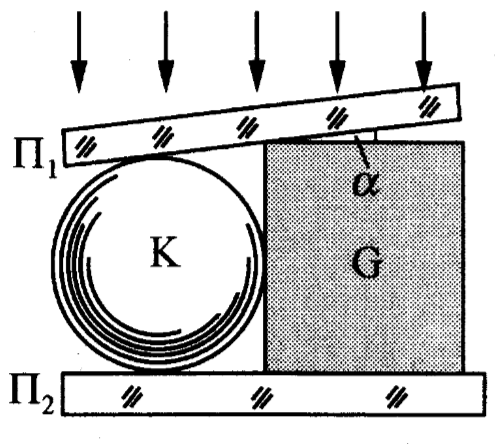
\includegraphics[width=0.55\textwidth]{2-8.png} % figure/image1.png
        \caption{测定滚珠直径}
    \end{minipage}
    \hfill
    % 第二张图
    \begin{minipage}[b]{0.45\textwidth}
        \centering
        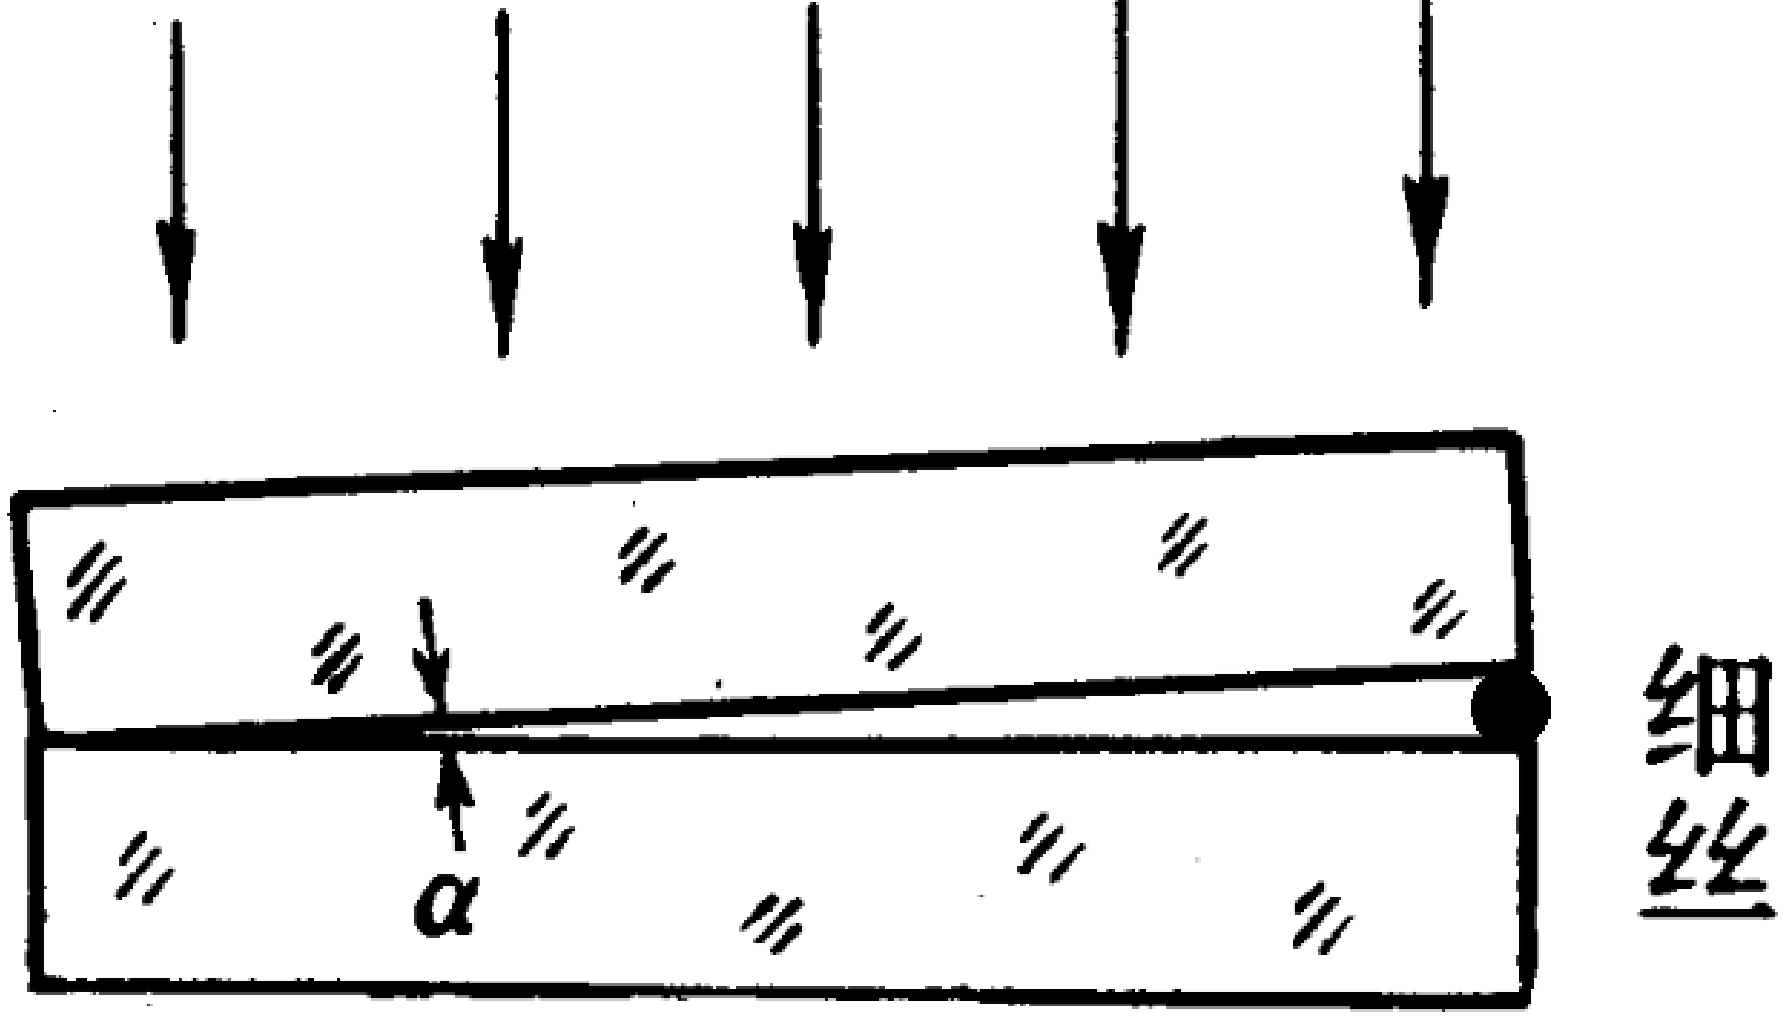
\includegraphics[width=0.55\textwidth]{2-9.png} % figure/image2.png
        \caption{测量细丝直径}
    \end{minipage}
\end{figure}

劈尖厚度的微小变化或者劈角的微小变化, 均将引起表面条纹发生显著的变化. 设想我们整体将上平板向上平移, 此时劈角不变, 因此条纹间距不会发生变化, 而是干涉条纹整体发生平移. 为了考察平移的方向, 我们选择考察具有固定光程差的条纹的位置. 如图所示, 假定交棱在左边, 则此种情况下, 具有相同光程差的位置将想左移动, 同样的分析可以得到, 条纹整体平移总是向着楔形交棱那一方. 当膜厚度增加时, 其定量关系是, 若条纹移动过$N$条, 则厚度变化是:
\[
\Delta h = \frac{N\lambda}{2}
\]

\insertfig{2-10.png}{劈尖条纹可能的移动示意图}{0.4}

下面来看牛顿环. 其装置如图所示. 一个曲率半径较大的透镜, 放置于一玻璃平板上, 便形成一空气薄膜, 其等厚线是一系列以接触点为中心的圆, 干涉图样如图.

\begin{figure}[htbp]
    \centering
    % 第一张图
    \begin{minipage}[b]{0.45\textwidth}
        \centering
        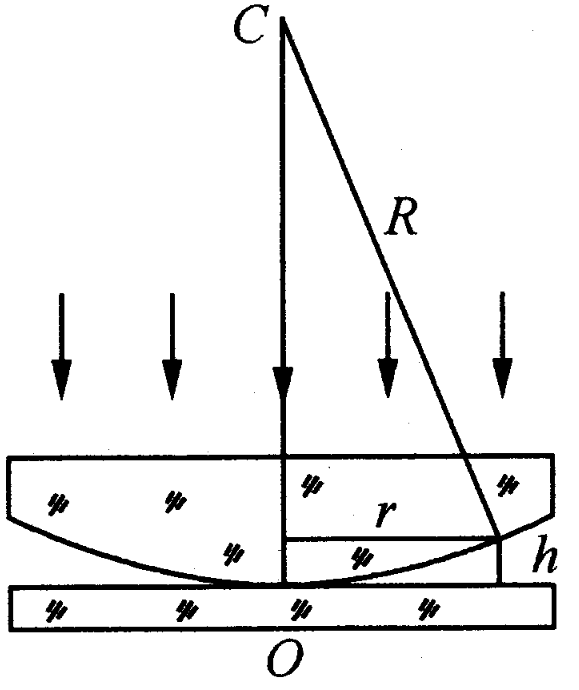
\includegraphics[width=0.55\textwidth]{2-11.png} % figure/image1.png
        \caption{牛顿环装置图}
    \end{minipage}
    \hfill
    % 第二张图
    \begin{minipage}[b]{0.45\textwidth}
        \centering
        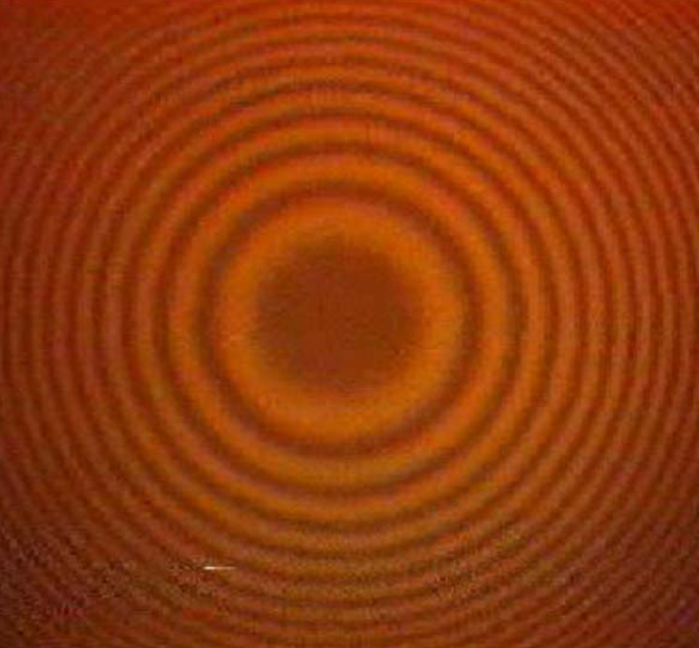
\includegraphics[width=0.55\textwidth]{2-12.png} % figure/image2.png
        \caption{牛顿环干涉图样}
    \end{minipage}
\end{figure}

若中心点与平板玻璃密接, 则中心点膜厚度为$0$, 中心为零级暗纹. 由此向外计算, 设第$k$级暗环的半径为$r_k$, 对应膜厚为$h_k$, 则满足:
\[
2nh_k = k\lambda_0
\]
几何关系有:
\[
R^2 = r_k^2+(R-h)^2 \Rightarrow r_k^2 = (2R-h_k)h_k \approx 2Rh_k
\]
因此得到($n=1$时为空气膜):
\[
r_k = \sqrt{\frac{kR\lambda_0}{n}}
\]
这样, 通过测量某一环的半径$r_k$和由其向外数第$m$环的半径为$r_{k+m}$, 据此, 可以算出透镜曲率半径:
\[
R = \frac{n(r_{k+m}^2-r_k^2)}{m\lambda_0} = \frac{n(d_{k+m}^2-d_k^2)}{4m\lambda_0}
\]

\insertfig{2-13.png}{利用牛顿环的变动指导透镜研磨}{0.4}

在光学冷加工车间, 常常利用牛顿环及其变动来快速检测透镜表面曲率是否合格以及下一步应该如何研磨. 如图, 标准件$G$覆盖于待测工件$L$上, 形成空气膜, 出现牛顿环. 圈数越多说明偏差越大, 当人们说某工件表面公差为一个光圈时, 就表示该工件与标准件之间的最大差距为$\frac{\lambda}{2}$. 有经验的工人只要将标准件下压, 根据光圈的伸缩情况就可以判断进一步研磨的位置. 若光圈扩大(吐出), 说明相同厚度的位置外扩, 应该研磨中间; 反之若光圈收缩(缩进), 应该研磨两侧.

\subsection{等倾干涉}

现在我们研究在膜层厚度均匀, 点光源照明条件下无穷远处的干涉场.

\insertfig{2-14.png}{等倾干涉装置图及干涉图样}{0.8}

如图所示, 由点光源发出的一个光线, 经过此薄层上下表面反射, 恰好分为彼此平行的两条光线, 而相干于无穷远. 为了便于观测, 也为了能获取完整的干涉条纹, 实验上是将点光源设置在旁侧, 经由一块倾斜的半反射镜, 向下照射薄膜, 并用一个透镜接收, 将无穷远处的干涉场聚焦于其后焦面, 呈现出干涉圆环图样.

\insertfig{2-15.png}{等倾干涉光程差}{0.5}

等倾干涉的光程差可以套用前面的结论:
\[
\Delta L = 2nh\cos i
\]
这里$i$是与入射角$i_1$对应的膜内的折射角, 由于膜层光学厚度均匀, 因此光程差唯一地决定于倾角$i$. 这就是说等倾角的场点轨迹就是条纹的形状, 显然其在后焦面上表现为一个圆环.

考虑第$k$级暗纹, 我们有光程差公式:
\[
\Delta L = 2nh\cos i = k\lambda
\]
在角度变化不大时, 我们可以在两边取差值:
\[
-2nh\sin i \Delta i = \Delta k \lambda \Rightarrow \Delta i = -\frac{\Delta k \lambda}{2nh\sin i}
\]
上式表明, $i_k$越大, $\Delta i$越小, 倾角不大的时候, 可以近似地认为相邻条纹半径之差正比于倾角之差. 因此我们就说在干涉图样中离中心较远的地方的等倾条纹更加密集.

由前面的光程差公式可以知道, 干涉图样中心处$i\approx 0$,$\cos i \approx 1$, 光程差最大, 干涉级次最高. 由内而外干涉级次依次降低. 当我们减小膜的厚度时, 追踪某一固定级次的条纹, 发现为了达到相同的光程差, 必须相应地减小折射角, 因此该级次的圆环由外向内移动到折射角较小的地方, 从而在宏观上表现为干涉图样向内收缩, 中心处不断有环吞入, 中心环的干涉级次减小. 反之膜的厚度增大时表现为干涉图样向外扩张, 中心处不断有环吐出, 中心环的干涉级次增大.

下面来看等倾干涉的最重要应用之一, 迈克耳孙干涉仪.

\insertfig{2-16.png}{迈克耳孙干涉仪结构}{0.35}

如图所示, $M_1$,$M_2$是一对精密磨光的平面镜, $G_1$,$G_2$是完全相同的两块玻璃板, 其中$G_1$的背面镀了一层很薄的银膜, 使得从光源入射的光线在这里被分为为强度几乎相等的两部分, 反射光束射向$M_1$, 被反射回来后再次透过$G_1$到达观测者, 透射光束射向$M_2$, 被反射回来到达$G_1$镀银面再次反射到达观测者. 这样的两束光相干产生干涉图样. $G_2$的意义在于补偿反射光比投射光多走过的光程.

现在我们分析迈克耳孙干涉仪产生的干涉图样. 干涉仪产生的图样可以被等效为$M_1$与$M_2'$镜面形成的空气层反射所产生的干涉场. 这里$M_2'$是右方$M_2$镜面对$G_1$镀银面反射而生成的像, 因此整体的干涉可以等效于空气膜形成的薄膜干涉. 具体的干涉图样我们如下给出, 具体的分析留给读者完成.

\insertfig{2-18.png}{干涉仪中的干涉图样}{0.5}


\insertfig{2-17.png}{产生对应干涉图样的等效空气膜}{0.5}

迈克耳孙干涉仪的一个重要应用是精密测长. 当$M_2$在折射率为$n$的介质中沿光轴平移长度为$l$时, 光程改变量为$2nl$, 设某处干涉强度变化了$N$次(吞入或吐出$N$个条纹), 则有:
\[
N \lambda_0 = 2nl \Rightarrow l = \frac{N\lambda_0}{2n}
\]

另一个重要应用是测量双线的波长差. 设用于照明的光源由两种波长为$\lambda_1$和$\lambda_2$的光合成的. 假定在初始某位置$\lambda_1$的亮纹与$\lambda_2$的暗纹相重合, 那么此时条纹最为模糊:
\[
\frac{\Delta L}{\lambda_1}-\frac{\Delta L}{\lambda_2}=k+\frac12,\qquad k\in\mathbb Z
\]
增加光程差, 直到下一次视场再次变得最为模糊时, 有:
\[
\Delta L_{\mathrm{beat}}\simeq\frac{\lambda_1\lambda_2}{|\lambda_1-\lambda_2|}=2d
\]

其中$d$为相邻两次条纹可见度极小位置之间镜子移动的距离, $\lambda$为两波长接近时的平均值. 由两组条纹的相对相位每改变$2\pi$出现一次可见度极小, 得到:
\[
\Delta\lambda=|\lambda_1-\lambda_2|=\frac{\lambda_1\lambda_2}{2d}\simeq\frac{\lambda^2}{2d}
\]

\section{光场的时间相干性}

在第一章中, 我们曾经提到过定态波的概念. 光源是一个由大量原子随机发射的光波列构成的集合. 每个原子由激发态跃迁到基态时, 会发出特定波长的光. 由于更加精细的原子结构的影响, 即便是同种原子也并不会都跃迁到相同的激发态, 导致光源发出的光并不是严格单色的, 而是具有一定的谱宽度, 也即波长位于一个以$\lambda$为中心的区间内.

\insertfig{2-19.png}{单色光的实际物理图像}{0.5}

波列指的是一列长度有限的波的扰动. 考虑光源每次发光的持续时间为$\Delta t$, 则波列在真空中的长度为$\Delta x = c\Delta t$. 而波列长度与波长谱的宽度有一反比关系, 其可以被表示为:
\[
\Delta x \cdot \Delta \lambda = \lambda^2
\]
关于这式子的由来有兴趣的读者可以参阅本节末尾的注记.

下面我们来看看什么是时间相干性. 考虑从同一光源在某一时刻发出的一个波列, 其经过某种装置后被分为两列相干波列, 这样被分开的两个波列之间是相干的, 因为其具有恒定的相位差. 只有这两列波在相近的时间内到达空间中的交叠光场, 在我们考察的空间区域内才能发生干涉, 否则看似相干的两束光, 由于实际上来自于光源发出的不同波列, 无法保证恒定的相位差, 就观察不到干涉现象. 这种因为光源的发光时间导致的干涉消失现象被称为光的时间相干性.

\insertfig{2-20.png}{波列长度与实际光程差的比较}{0.4}

如图所示设光程差为$\delta$, 考虑可能发生干涉的两个光波列. $\delta=0$时, 两波列在时间上完全重叠, 干涉条纹的可见度最大. 光程差小于波列长度但不为$0$, 干涉条纹仍然可见. 当光程差超过相干长度, 条纹可见度通常很低; 其具体变化取决于光源的光谱形状. 迈克耳孙干涉仪中的补偿板就有一作用是为了防止两列波的光程差过大而无法被观测到相干现象.

可用条纹可见度下降的特征尺度来定义相干长度; 具体数值取决于光谱形状和采用的判据. 这样根据我们前面给出的反比关系式$\Delta x \cdot \Delta \lambda = \lambda^2$, 得到相干长度的表达式为:
\[
\delta_m = \frac{\lambda^2}{\Delta \lambda}
\]
我们可以发现时间相干性是与光谱的单色性强相关的, 光谱的单色性越好, $\Delta \lambda$越小, 相干长度越长, 时间相干性越好.

\begin{noteenv}
    我们先引入光源发光的光强谱密度概念. 我们采用波数来表征光的单色性. 设光源发出的光中, 在$k \sim k+\Delta k$中含有的光强是:
    \[
    \Delta I_0 = i(k)\cdot \Delta k
    \]
    取极限得到微分形式:
    \[
    \d I_0 = i(k)\d k, \quad i(k)= \frac{\d I_0}{\d k}
    \]
    这样$i(k)$就被称作入射光的光强谱密度函数, 其物理意义是在波数$k$附近单位波数间隔内入射光中所含的光强. 为了计算简明, 我们采取一个简化模型, 设光强的谱密度函数有如下的形式:
    \[
    i(k)=
    \begin{cases}
    i_0, & |k-k_0|\le \frac{\Delta k}{2} \\
    0, & otherwise
    \end{cases}
    \]
    考虑谱元$k \sim k+\d k$. 在这个谱元中各光束发生干涉, 其干涉叠加强度为:
    \[
    \d I = \d I_0 (1+\cos k\Delta L)=i(k)(1+\cos k\Delta L)\d k
    \]
    总强度是各谱元贡献的非相干叠加, 因为各谱元之间频率不同:
    \[
    I = \int_0^{\infty}i(k)(1+\cos k \Delta L)\d k
    \]
    同时注意到:
    \[
    \int_0^{\infty} i(k)\d k = I_0
    \]
    这是入射光总强度, 于是有:
    \[
    I(\Delta L) = I_0+\int_0^{\infty}i(k)\cos (k\Delta L)\cdot \d k
    \]
    这是一个由任意的谱密度函数求解总光强的积分式, 代入我们选择的谱函数, 得到:
    \[
    I(\Delta L)=i_0\Delta k+i_0\int_{k_1}^{k_2}\cos (k \Delta L)\d k = I_0(1+\frac{\sin v}{v}\cos k_0 \Delta L)
    \]
    其中$v =\frac{\Delta k\Delta L}{2}$

    与一般的干涉公式对比, 我们发现后面的干涉项受到了$\frac{\sin v}{v}$的调制, 因此当$v = \pi$时干涉项为$0$, 条纹可见度为$0$, 此时有:
    \[
    \Delta k \cdot \frac{\Delta L}{2} = \pi \Rightarrow \Delta L_{\max} = \frac{2\pi}{\Delta k}
    \]
    注意到波数与波长的关系:
    \[
    k = \frac{2\pi}{\lambda} \Rightarrow \Delta k = \frac{2\pi}{\lambda^2}\Delta \lambda
    \]
    代入上式, 就得到:
    \[
    \Delta L_{\max} = \frac{\lambda^2}{\Delta \lambda}
    \]
    这样我们得到了由单色性导出的最大光程差公式. 根据时间相干性中的讨论, 这个最大光程差应该与波列长度相等, 于是有:
    \[
    \Delta x =\frac{\lambda^2}{\Delta \lambda} \Rightarrow \Delta x \cdot \Delta \lambda = \lambda^2
    \]
\end{noteenv}

